\chapter{Experiments and Results}
\todo{Alternative titles: Capabilities of LSTMs, Strengths and Weaknesses of LSTM, Analysis of LSTMs, The LSTM: A Analysis}

	The aim of this chapter is to develop an understanding of how the recurrent neural networks work, specifically the LSTM.
	We begin with a very simple memorization task to demonstrate how an LSTM is trained on sequences of data and what effect different hyperparameters have.
	Building on this knowledge, we explore more sophisticated tasks such as predicting the motion of a cloud of points which will finally lead into the challenging problem of visual odometry and structure from motion.
	
	\section{A First Toy Example: Memorizing Digits}
		% Capabilities of LSTM
		% - Memory: Describe binary memory example (sequence of binary digits)
		% - As classification, formula for cross-entropy loss
		% - All formulas for LSTM (gates etc.)
		% - What is the purpose of Hidden size for remembering sequence
		% - What would one possible solution for the LSTM weights?
		% - 
		
		%To understand how LSTMs are used to learn from sequences of data and how their memory works, we conduct a small example for demonstration. 
		This first experiment is to show the capabilities and limitations of the LSTM.
		Can it memorize the past and use this knowledge for future outputs?
		And how far back in time can it remember?
		Does it work best for classification or regression?
		\todo{Regression still missing from experiments! (one fig. generated)}
		These are the main questions that are investigated in this section.
		
		\paragraph{The Task}
		The goal is to train an LSTM that remembers the last $m$ digits of a random sequence of binary digits $\vectr{x}_t \in \{0, 1\}$. 
		Thus, at time $t$ we would like the output to be the digit $\vectr{x}_{t-m}$ that was fed $m$ time steps before. 
		For example, here are two sequences of zeros and ones shifted by $m = 3$:
		\newcommand{\hlc}[2][yellow]{{%
				\colorlet{foo}{#1}%
				\sethlcolor{foo}\hl{#2}}%
		}
		\begin{center}
			\texttt{\dots01\hlc[pink]{1}\hlc[green!45]{1}\hlc[cyan!50]{0}10110\dots}
			\\
			\texttt{\dots00101\hlc[pink]{1}\hlc[green!45]{1}\hlc[cyan!50]{0}10\dots}
		\end{center}
		The first line is the input sequence and below is the desired output sequence.
		The LSTM reads the digits one by one to store them in memory and at the same time it outputs the digit from memory at time $t - 3$ as highlighted by the colors above.
		%How can we model and train this sequence-to-sequence problem?
		
		In order to tackle a machine learning problem, one needs to define three key elements:
		\begin{enumerate}
			\item Model
			\item Performance measure
			\item Optimization procedure
		\end{enumerate}
	
		\paragraph{The Model}
		We begin by defining the model.
		The first part of our model is the LSTM itself as it was defined in equations~\ref{eq:LSTM_recurrence} and~\ref{eq:Vanilla-LSTM-Definition}.
		Since the output can only be two numbers (zero and one), we will treat the problem as a classification task.
		To do this, we add an affine layer to shrink the size of the LSTM output $\vectr{h}_t$ down to a two-element vector
		\begin{equation}
			\vectr{z}_t = \matr{V} \vectr{h}_t + \vectr{c}.
		\end{equation}
		The last layer is the \emph{softmax} operation
		\begin{eqnarray}
			\text{softmax}(\vectr{x})_j = \frac{e^{x_{j}}}{\sum_{k=1}^{K} e^{x_{k}}},  & & j = 1, \dots, K
		\end{eqnarray}
		which is applied to $\vectr{z}_t$, where $K = 2$ in this example.
		The softmax layer forces the output to be a probability vector, which means that each entry is in the range $[0, 1]$ and all elements sum to one.
		Therefore, the output vector contains two probabilities, 
		\begin{equation*}
			\vectr{p}_t = 
			\begin{bmatrix}
				P(\vectr{o}_t = 0 \mid \vectr{x}_t, \vectr{h}_{t - 1}, \vectr{c}_{t - 1}) \\ 
				P(\vectr{o}_t = 1 \mid \vectr{x}_t, \vectr{h}_{t - 1}, \vectr{c}_{t - 1})
			\end{bmatrix}.
		\end{equation*}
		The output digit $\vectr{o}_t$ must be chosen according to the highest probability.
		A summary of the full model is shown in table~\ref{tbl:model_classification_binary_digits}.
		\begin{table}[tb]
			\small
			\begin{center}
				\begin{tabular}{|l|c|c|c|c|}
					\hline
					Layer 	& Variable 			& Input size 	& Output size 	& Parameters 			\\ \hline
					LSTM 	& $\vectr{h}_t$		& 1 			& $d$ 			& $4d(d + 1) + 4d$ 		\\ \hline
					Affine 	& $\vectr{z}_t$		& $d$ 			& 2 			& $2d + 2$ 				\\ \hline
					Softmax & $\vectr{p}_t$		& 2 			& 2 			& 0						\\ \hline
				\end{tabular}
			\end{center}
			\caption[A simple model to memorize a binary sequence]
					{A simple model to memorize a binary sequence. 
					 The variable $d$ is the hidden size of the LSTM.}
			\label{tbl:model_classification_binary_digits}
		\end{table}
		
		\paragraph{The Performance Measure}
		Next, we have to define a suitable loss function. 
		For classification with softmax as the last layer, it is preferable to use the negative log-likelihood
		\begin{equation}
			L(\vectr{x}, y) = -\log\left(\vectr{x}_y\right)
		\end{equation}
		as a loss function. 
		Here, the first argument of $L$ would be replaced with the output $\vectr{p}_t$ of the network and the second argument is the ground truth label. 
		Since we are predicting the digit from $m$ time steps ago, the ground truth directly comes from the input sequence, and therefore the label $y_t$ at time $t$ is the input $\vectr{x}_{t - m}$.
		By minimizing this loss, the probability for the correct class is maximized.
		As described in equation~\ref{eq:loss_for_rnn}, the total loss for the entire sequence is the sum over the individual losses.
		\todo{need better explanation of log-likelihood loss here}
		
		\paragraph{The Optimization Procedure}
		In order to use the loss function to update the model weights, one has to specify an optimization algorithm.
		One of the most general purpose optimization algorithms is \emph{gradient descent}, which can find a local minimum of a function $F$ by iteratively stepping in the opposite direction of the gradient, hence the update rule
		\begin{equation}
			\vectr{w} \leftarrow 
			\vectr{w} - \lambda \frac{\partial F(\vectr{w})}{\partial \vectr{w}}.
		\end{equation}
		The parameter $\vectr{w}$ converges to a local minimum when a suitable learning rate $\lambda$ is chosen.
		
		In the context of this experiment, $\vectr{w}$ are the model parameters and $F$ is the loss over the training data. 
		One possible update rule is
		\begin{equation}
			\vectr{w} \leftarrow 
			\vectr{w} - \lambda 
			\sum_{i}
			\sum_{t = 1}^{T}
			\frac{\partial L(f_{\vectr{w}}(\vectr{x}_t^{i}), \vectr{x}_{t - m}^{i})}{\partial \vectr{w}}, 
		\end{equation}
		where $\vectr{x}_t^{i}$ denotes the input at time $t$ of the $i$-th sequence.
		Because this experiment is completely artificial, it is possible to generate as much data as needed.
		Instead of generating many smaller sequences, one can generate a single large sequence or sample the digits on-the-fly.
		In order to save memory and reduce computation, one can choose to limit the gradient computation through time.
		This is called \emph{truncated backpropagation through time (TBPTT)}. 
		Starting from the beginning of the sequence, $T$ inputs are fed to the LSTM followed by the loss computation.
		The gradient computation is performed for exactly $T$ steps back in time and the weights are updated accordingly. 
		Continuing with this pattern, the next $T$ inputs are fed for the next update and so on.
		In each step, the hidden state is carried over from the previous digit.
		This way, there is always information available from the past even though the gradients are never propagated to the very beginning of the sequence.
		\todo{Explain this in the theoretical section, also explain how (truncated) backpropagation works for LSTM}
		
		\paragraph{Results for Binary Sequence}
		Now that task, model and optimization procedure are defined, the model can be trained and evaluated.
		For all experiments, we train the model and test on new unseen data of the same size by computing the accuracy, that is the relative frequency of correctly predicted digits.
		First, let's train and evaluate on the simplest model possible: The LSTM has a hidden size of one ($d = 1$).
		\begin{figure}[tb]
			\centering
			\begin{subfigure}[b]{0.5\linewidth}
				\centering
				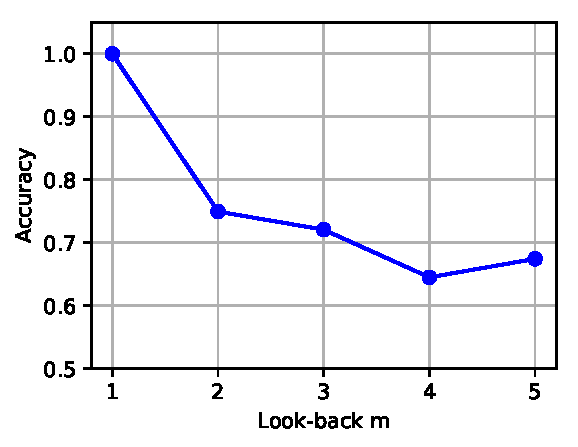
\includegraphics[width=\linewidth]{Images/Python-Plots/memory/accuracy-vs-look-back}
				\caption{
					$d = 1, T = 50, \lambda = 0.01, N = 10^5$
					\label{fig:accuracy-vs-look-back}
				}
			\end{subfigure}%
			\begin{subfigure}[b]{0.5\linewidth}
				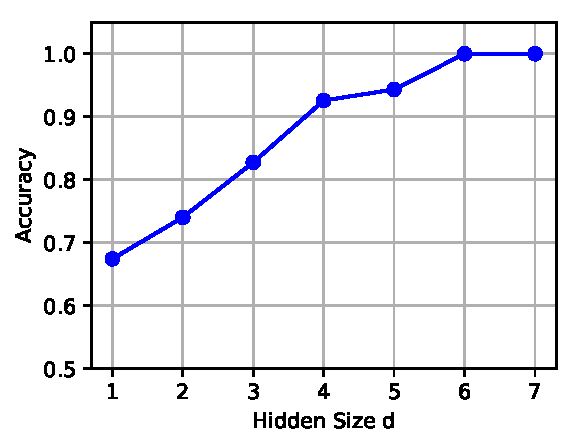
\includegraphics[width=\linewidth]{Images/Python-Plots/memory/accuracy-vs-hidden-size}
				\caption{
					$m = 5, T = 50, \lambda = 0.01, N = 10^5$
					\label{fig:accuracy-vs-hidden-size}
				}
			\end{subfigure}
			\\
			\begin{subfigure}[b]{0.5\linewidth}
				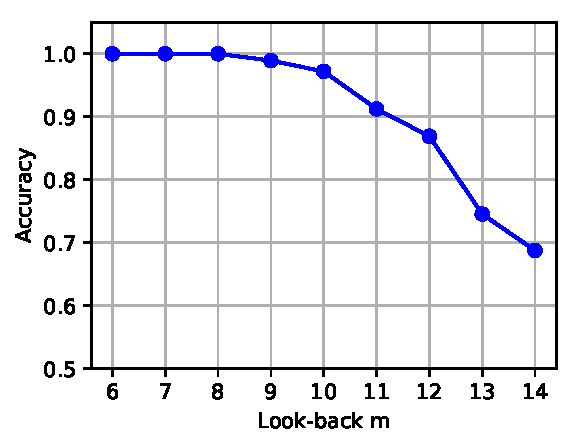
\includegraphics[width=\linewidth]{Images/Python-Plots/memory/accuracy-vs-look-back2}
				\caption{
					$d = 50, T = 50, \lambda = 0.001, N = 10^5$
					\label{fig:accuracy-vs-look-back2}
				}
			\end{subfigure}%
			\begin{subfigure}[b]{0.5\linewidth}
				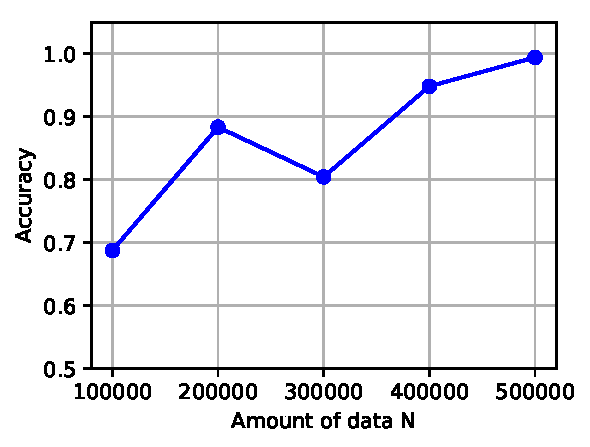
\includegraphics[width=\linewidth]{Images/Python-Plots/memory/more-training-data}
				\caption{
					$m = 14, d = 50, T = 50, \lambda = 0.001$
					\label{fig:more-training-data}
				}
			\end{subfigure}
			\caption[Memorizing the past with the LSTM: Binary digits]
			{Accuracy on the test dataset for varying parameters while keeping others fixed. 
				The parameters involved are the hidden size $d$, look-back $m$, BPTT $T$, training set size $N$ and learning rate $\lambda$. 
				(a) The hidden size is too small.
				(b) Effect of increasing the hidden size.
				(c) Only increasing the hidden size is not enough.
				(d) Increasing the amount of training data.}
			\label{fig:ablation-study-binary-memory}
		\end{figure}
		The result is shown in figure~\ref{fig:accuracy-vs-look-back}. 
		We observe that the model can perfectly memorize the digit of one time step in the past ($m = 1$).
		However, when increasing the look-back the accuracy drops significantly.
		This problem can be fixed by increasing the hidden size as shown in~\ref{fig:accuracy-vs-hidden-size}.
		Based on these observations, it seems that the hidden size $d$ is related to the memory capacity of the network and must always be chosen higher than the look-back $m$. 
		But this hypothesis does not hold true when we continue to increase $m$ as demonstrated in~\ref{fig:accuracy-vs-look-back2}.
		Figure~\ref{fig:more-training-data} shows that for higher look-back, we also need significantly more training data. 
		
		\paragraph{Extension to Multi-class}
		So far we have learned a binary classifier, but we can extend the task to go beyond that to make the problem harder.
		Instead of having only two symbols 0 and 1, we can choose each digit to be a number $\vectr{x}_t \in \{1, \dots, C\}$.
		This is essentially a classification problem with $C$ classes.
		The updated model is shown in table~\ref{tbl:model_classification_multi_class_digits}.
		\begin{table}[tb]
			\small
			\begin{center}
				\begin{tabular}{|l|c|c|c|c|}
					\hline
					Layer 	& Variable 			& Input size 	& Output size 	& Parameters 			\\ \hline
					LSTM 	& $\vectr{h}_t$		& 1 			& $d$ 			& $4d(d + 1) + 4d$ 		\\ \hline
					Affine 	& $\vectr{z}_t$		& $d$ 			& $C$ 			& $Cd + C$ 				\\ \hline
					Softmax & $\vectr{p}_t$		& $C$ 			& $C$ 			& 0						\\ \hline
				\end{tabular}
			\end{center}
			\caption[A simple model to memorize a sequence of numbers]
					{A simple model to memorize a sequence of numbers.
					 This is a generalization of the binary model in table~\ref{tbl:model_classification_binary_digits} where $C = 2$.}
			\label{tbl:model_classification_multi_class_digits}
		\end{table}
		The model is trained and evaluated for each value $C \in \{1, \dots 15\}$.
		\begin{figure}[tb]
			\centering
			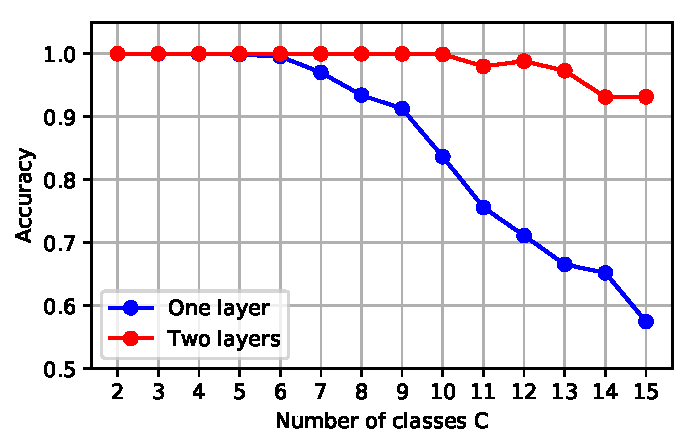
\includegraphics[width=0.7\linewidth]{Images/Python-Plots/memory/accuracy-vs-multiple-classes-and-layers}
			\caption[Memorizing the past with the LSTM: Multiple classes]
					{Memorizing multiple classes with LSTM.
					 Performance of single layer LSTM vs. stacked LSTM.
					 Adding more layers helps deal with the higher complexity of the output.
					 Hyperparameters: $m = 5, d = 50, T = 50, \lambda = 0.001, N = 10^5$.
					 }
			\label{fig:accuracy-vs-multiple-classes-and-layers}
		\end{figure}
		The blue line in figure~\ref{fig:accuracy-vs-multiple-classes-and-layers} shows that the accuracy decreases the more classes are used in the sequence.
		This is due to the more complex mapping between input and output. 
		An LSTM with a single layer can not handle the complexity.
		As shown in the red line in figure~\ref{fig:accuracy-vs-multiple-classes-and-layers}, adding a second layer boosts the performance.
		
		
	\section{Tracking a Moving Point Cloud}
		
		Up to this point, the input to the LSTM was always one-dimensional (a number/digit).
		But how well can it handle vectors as input?
		This is the main question for this section.
		To explore it, we conduct a synthetic experiment for a moving camera.
		
		\paragraph{The Task}
		In this next experiment we would like to study the capabilities of the LSTM on a task for motion estimation.
		To do so, we generate a few 3D points and project them into the image plane of a moving camera.
		This will create an animation of a set of 2D points.
		
		\begin{figure}[tb]
			\centering
			\includegraphics[width=0.7\linewidth]{example-image-a}
			\caption[]
					{\todo{point cloud example, show few points and multiple points}}
			\label{}
		\end{figure}
	
		\paragraph{The Data}
		Each sample from the dataset is a synthetic sequence of frames seen by a moving camera in front of a cloud of 3D points.
		There are two main steps involved in generating the data.
		First, we generate the 3D points.
		Second, the points need to be projected to the screen of each camera.
		The camera is moving left and right to create a simple motion.
		To create a large and diverse dataset, we can generate many such sequences for different point clouds and horizontal motions.
		
		To make this experiment very simple, the points are distributed uniformly on the surface of a sphere.
		This can be done by sampling two random variables $z \sim \mathcal{U}(-1, 1)$ and $\theta \sim \mathcal{U}(0, 2\pi)$ that can be used to parameterize the point
		\begin{equation}
			\vectr{p} = 
			\begin{bmatrix}
				\sqrt{1 - z^2} \cos(\theta) \\ 
				\sqrt{1 - z^2} \sin(\theta) \\
				z
			\end{bmatrix}
		\end{equation}
		on the unit sphere. 
		After repeating this $M$ times, we obtain a cloud $C = \{\vectr{p}_1, \dots \vectr{p}_M\}$ with $M$ points.
		Each of these points has to be projected
		
		
		\paragraph{The Model}
		
		\paragraph{The Optimization Procedure}
		
		\paragraph{Results}
		
		\paragraph{}
		
		